% See exam.cls and examdoc.tex for the license information
\documentclass[12pt, answers]{exam}

\usepackage{amssymb}
\usepackage{makeidx}
\usepackage{amsmath}
\usepackage{graphicx}
\usepackage{caption}
\usepackage{tabulary}
\usepackage{color}
\usepackage{multicol}
\usepackage{multirow}
\usepackage{enumerate}
\usepackage{float}
\usepackage{colortbl}
\usepackage[table,xcdraw]{xcolor}

\usepackage{array}
\newcolumntype{C}[1]{>{\centering\let\newline\\\arraybackslash\hspace{0pt}}m{#1}}

\addpoints

% In case we're not using hyperref.sty:
\providecommand{\texorpdfstring}[2]{#1}
% The following can be used in \section commands
% without generating pdf warnings:
\newcommand{\bs}{\texorpdfstring{\char`\\}{}}

\makeindex

\newcommand{\indc}[1]{\index{#1@\texttt{\char`\\#1}}}
\newcommand{\indcsub}[2]{\index{#1@\texttt{\char`\\#1}!#2}}
\newcommand{\indcstart}[1]{\index{#1@\texttt{\char`\\#1}|(}}
\newcommand{\indcstop}[1]{\index{#1@\texttt{\char`\\#1}|)}}

\newcommand{\indt}[1]{\index{#1@\texttt{#1}}}
\newcommand{\indtsub}[2]{\index{#1@\texttt{#1}!#2}}
\newcommand{\indtstart}[1]{\index{#1@\texttt{#1}|(}}
\newcommand{\indtstop}[1]{\index{#1@\texttt{#1}|)}}

\extraheadheight{-.4in}

\pagestyle{headandfoot}
%\extraheadheight{.2 in}
\firstpageheader{}{}{}
\runningheader{}{}{}
\firstpagefooter{INF281}{Exercise 06}{Page \thepage\ of \numpages}
\firstpagefootrule
\runningfooter{INF281}{Exercise 06}{Page \thepage\ of \numpages}
\runningfootrule

%---------------------------------------------------------------------

\shadedsolutions
%\noprintanswers
\definecolor{SolutionColor}{rgb}{0.8,0.9,1}
\newcommand{\mybox}[1]{\par\noindent\colorbox{SolutionColor}
{\parbox{\dimexpr\textwidth-2\fboxsep\relax}{#1}}}

\begin{document}

\section*{INF281 Exercise 06 solutions}

%---------------------------------------------------------------------
\begin{questions}

%%% Question 1
\question \textbf{SP score}

The SP (sum-of-pairs) score is used to evaluate multiple sequence alignments.
 
\[
S(\mathcal{A}) = \sum_{i=1}^{m-1} \sum_{j=i+1}^{m} S(\bar{s}^i, \bar{s}^j)
\]

Use the simple scoring scheme and the alignment $\mathcal{A}$ to answer the following questions.

\begin{multicols}{2}
Alignment $\mathcal{A}$:
\begin{verbatim}
  Seq1: A-G
  Seq2: GCG
  Seq3: G-T
\end{verbatim}
\vfill\null
\columnbreak

\noindent Scoring scheme: \\ 
\null \quad $R_{ab}$ = 1 for a = b \\ 
\null \quad $R_{ab}$ = 0 for a $\neq$ b \\ 
\null \quad g = 1

\end{multicols} 

\textbf{N.B.} The score of a column with two blanks in a pairwise alignment should be 0.

\vspace{0.1 in}

\begin{parts}

%% (a)
  \part Calculate the pairwise score $S(\bar{s}^1, \bar{s}^2)$.
  
\begin{solution}[0.35 in]
0
\end{solution}

%% (b)
  \part Calculate the pairwise score $S(\bar{s}^1, \bar{s}^3)$.

\begin{solution}[0.35 in]
0
\end{solution}

%% (c)
  \part Calculate the pairwise score $S(\bar{s}^2, \bar{s}^3)$.
  
\begin{solution}[0.35 in]
0
\end{solution}

%% (d)
  \part Calculate the SP score $S(\mathcal{A})$.

\begin{solution}[0.35 in]
$0 + 0 + 0 = 0$ 
\end{solution}

\end{parts}



%%% Question 2
\question \textbf{Tree topology}

A rooted phylogenetic tree can have three topologically different trees when $m$ is 3.

\begin{parts}

\vspace{0.1 in}

%% (a)
  \part  Fill the labels A, B, or C to satisfy three topologically distinct trees.
  
\begin{figure}[H]
      \centering
      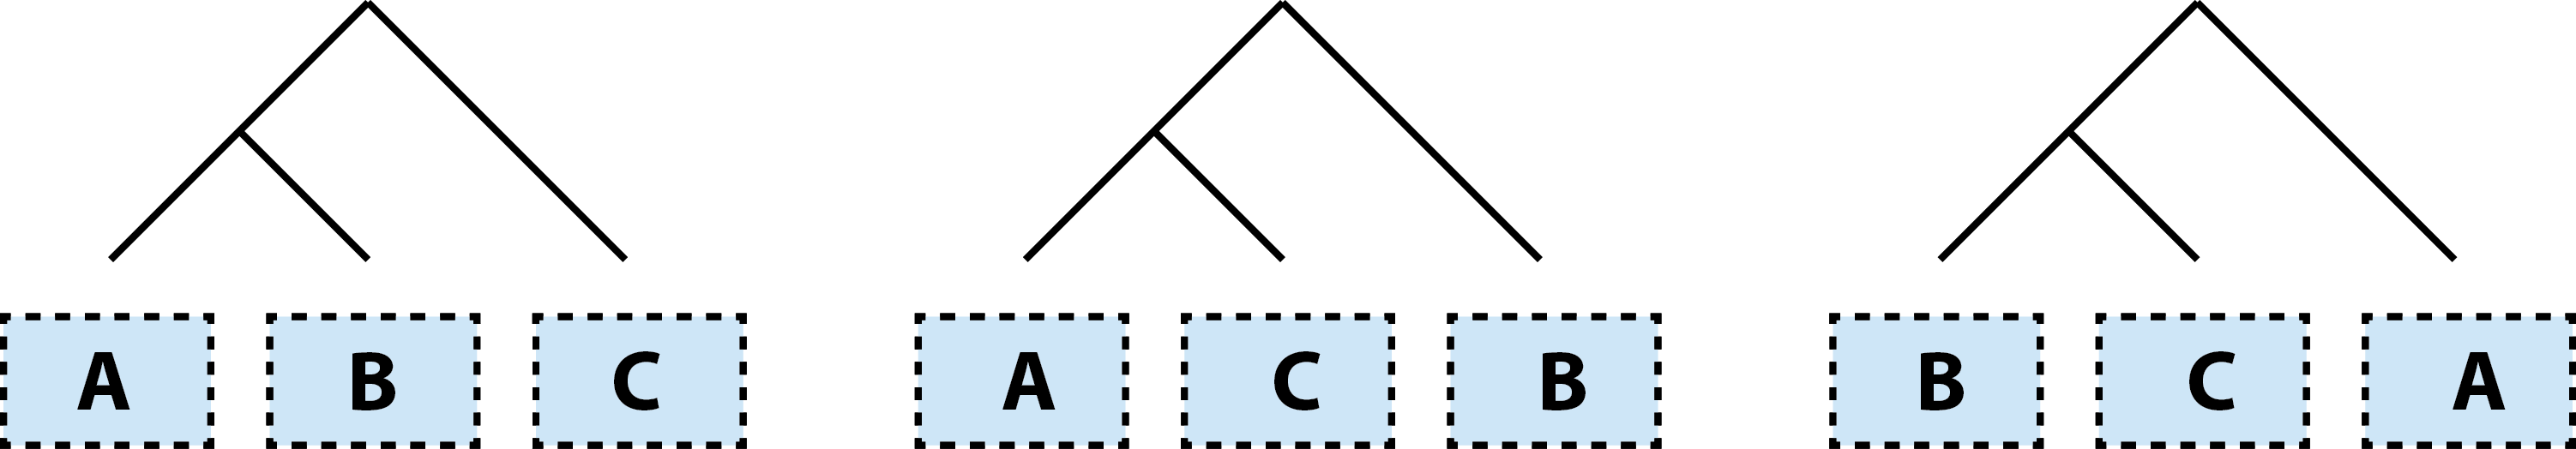
\includegraphics[width=0.7 \textwidth]{fig09/tree_topology_solution.png}
\end{figure}

\end{parts}


\newpage

%%% Question 3
\question \textbf{UPGMA}

UPGMA is an unweighted version of PGMA (pair-group method using arithmetic mean) for reconstructing a phylogenetic tree. Pairwise sequence alignments are used to calculate the distances among four sequences A, B, C, and D.

\begin{table}[H]
\centering
\begin{tabular}{lllll}
                       & A                      & B                      & C                      & D                      \\ \cline{2-5} 
\multicolumn{1}{l|}{A} & \multicolumn{1}{l|}{0} & \multicolumn{1}{l|}{2} & \multicolumn{1}{l|}{7} & \multicolumn{1}{l|}{7} \\ \cline{2-5} 
B                      & \multicolumn{1}{l|}{}  & \multicolumn{1}{l|}{0} & \multicolumn{1}{l|}{5} & \multicolumn{1}{l|}{9} \\ \cline{3-5} 
C                      &                        & \multicolumn{1}{l|}{}  & \multicolumn{1}{l|}{0} & \multicolumn{1}{l|}{8} \\ \cline{4-5} 
D                      &                        &                        & \multicolumn{1}{l|}{}  & \multicolumn{1}{l|}{0} \\ \cline{5-5} 
\end{tabular}
\end{table}

Below are two examples of the distance calculation that can be used for UPGMA.

\[
d_{(\alpha\beta),\gamma}=\dfrac{d_{\alpha,\gamma} + d_{\beta,\gamma}}{2}
\]

\[
d_{(\alpha\beta\gamma),\delta}=\dfrac{d_{\alpha,\delta} + d_{\beta,\gamma} + d_{\delta,\gamma}}{3}
\]

\begin{parts}

\vspace{0.1 in}

%% (a)
  \part Identify the first internal node and update the distance matrix.
  
\begin{table}[H]
\centering
\begin{tabular}{
>{\columncolor[HTML]{CCE5FF}}c 
>{\columncolor[HTML]{CCE5FF}}c 
>{\columncolor[HTML]{CCE5FF}}c 
>{\columncolor[HTML]{CCE5FF}}c }
{\color[HTML]{000000} }                                                  & {\color[HTML]{000000} (AB)}                                           & {\color[HTML]{000000} C}                                              & {\color[HTML]{000000} D}                                              \\ \cline{2-4} 
\multicolumn{1}{c|}{\cellcolor[HTML]{CCE5FF}{\color[HTML]{000000} (AB)}} & \multicolumn{1}{c|}{\cellcolor[HTML]{CCE5FF}{\color[HTML]{000000} 0}} & \multicolumn{1}{c|}{\cellcolor[HTML]{CCE5FF}{\color[HTML]{000000} 6}} & \multicolumn{1}{c|}{\cellcolor[HTML]{CCE5FF}{\color[HTML]{000000} 8}} \\ \cline{2-4} 
{\color[HTML]{000000} C}                                                 & \multicolumn{1}{c|}{\cellcolor[HTML]{CCE5FF}{\color[HTML]{000000} }}  & \multicolumn{1}{c|}{\cellcolor[HTML]{CCE5FF}{\color[HTML]{000000} 0}} & \multicolumn{1}{c|}{\cellcolor[HTML]{CCE5FF}{\color[HTML]{000000} 8}} \\ \cline{3-4} 
{\color[HTML]{000000} D}                                                 & {\color[HTML]{000000} }                                               & \multicolumn{1}{c|}{\cellcolor[HTML]{CCE5FF}{\color[HTML]{000000} }}  & \multicolumn{1}{c|}{\cellcolor[HTML]{CCE5FF}{\color[HTML]{000000} 0}} \\ \cline{4-4} 
\end{tabular}
\end{table}

%% (b)
  \part Identify the second internal node and update the distance matrix accordingly.
  
\begin{table}[H]
\centering
\begin{tabular}{
>{\columncolor[HTML]{CCE5FF}}c 
>{\columncolor[HTML]{CCE5FF}}c 
>{\columncolor[HTML]{CCE5FF}}c }
{\color[HTML]{333333} }                                                   & {\color[HTML]{333333} (ABC)}                                          & {\color[HTML]{333333} D}                                              \\ \cline{2-3} 
\multicolumn{1}{c|}{\cellcolor[HTML]{CCE5FF}{\color[HTML]{333333} (ABC)}} & \multicolumn{1}{c|}{\cellcolor[HTML]{CCE5FF}{\color[HTML]{333333} 0}} & \multicolumn{1}{c|}{\cellcolor[HTML]{CCE5FF}{\color[HTML]{333333} 8}} \\ \cline{2-3} 
{\color[HTML]{333333} D}                                                  & \multicolumn{1}{c|}{\cellcolor[HTML]{CCE5FF}{\color[HTML]{333333} }}  & \multicolumn{1}{c|}{\cellcolor[HTML]{CCE5FF}{\color[HTML]{333333} 0}} \\ \cline{3-3} 
\end{tabular}
\end{table}

%% (c)
  \part Reconstrut a rooted tree from the calcualted distances.
  
\begin{figure}[H]
      \centering
      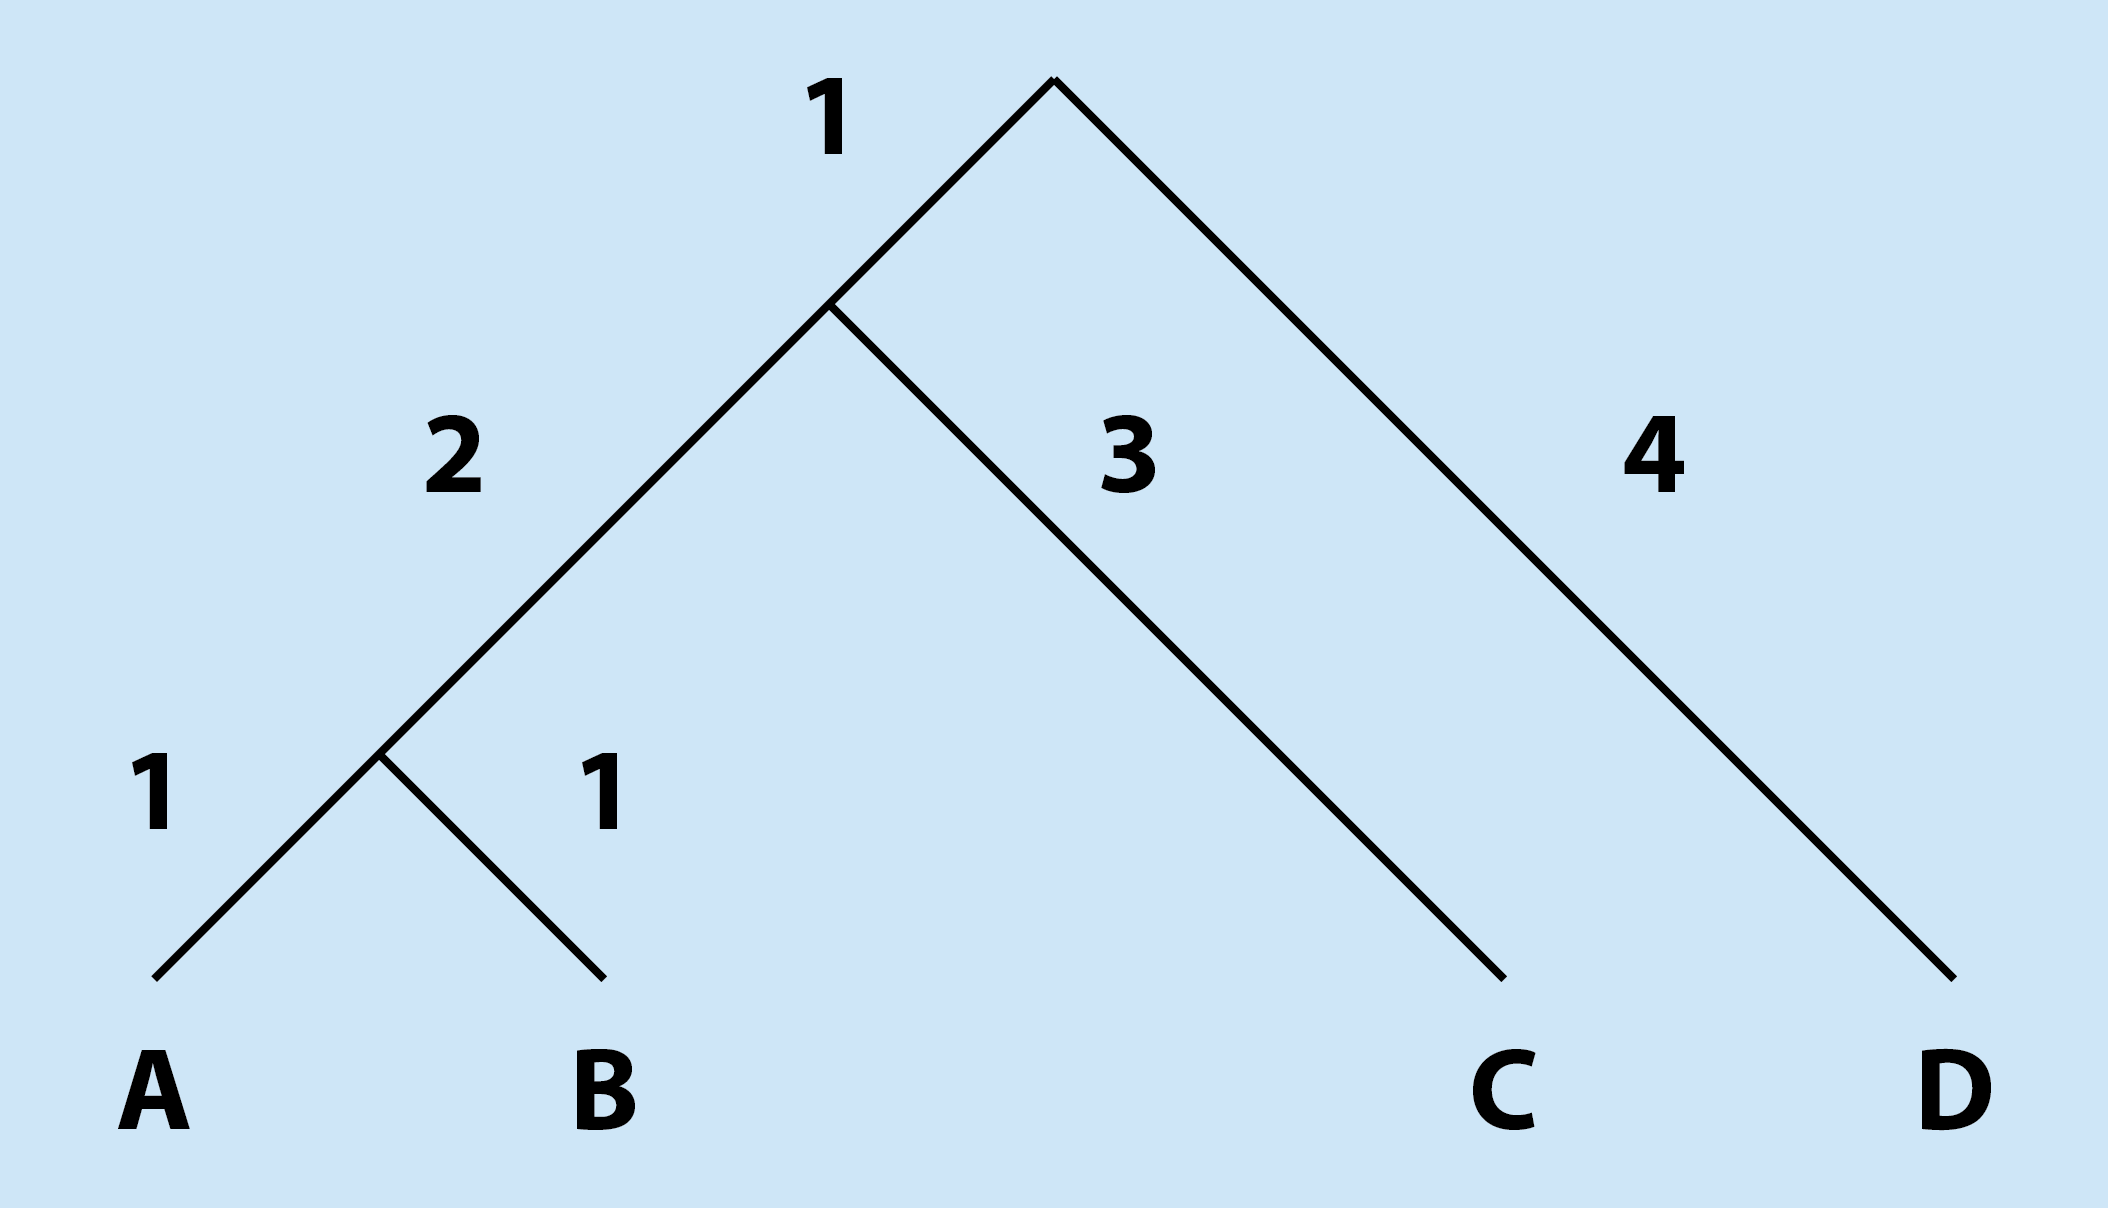
\includegraphics[width=0.3 \textwidth]{fig09/ultrametric_tree_solution.png}
\end{figure}
  
%% (d)
  \part Reconstruct a rooted tree by using UPGMA.
  
\begin{table}[H]
\centering
\begin{tabular}{lllll}
                       & A                      & B                                              & C                                              & D                                              \\ \cline{2-5} 
\multicolumn{1}{l|}{A} & \multicolumn{1}{l|}{0} & \multicolumn{1}{l|}{\cellcolor[HTML]{CCE5FF}2} & \multicolumn{1}{l|}{\cellcolor[HTML]{CCE5FF}6} & \multicolumn{1}{l|}{\cellcolor[HTML]{CCE5FF}8} \\ \cline{2-5} 
B                      & \multicolumn{1}{l|}{}  & \multicolumn{1}{l|}{0}                         & \multicolumn{1}{l|}{\cellcolor[HTML]{CCE5FF}6} & \multicolumn{1}{l|}{\cellcolor[HTML]{CCE5FF}8} \\ \cline{3-5} 
C                      &                        & \multicolumn{1}{l|}{}                          & \multicolumn{1}{l|}{0}                         & \multicolumn{1}{l|}{\cellcolor[HTML]{CCE5FF}8} \\ \cline{4-5} 
D                      &                        &                                                & \multicolumn{1}{l|}{}                          & \multicolumn{1}{l|}{0}                         \\ \cline{5-5} 
\end{tabular}
\end{table}

\end{parts}



%%% Question 4
\question \textbf{Maximum parsimony}

The maximum parsimony uses column-wise operations of union and intersection. The number of union operations is counted to find the tree that minimizes the evolutionary changes. \\

\begin{figure}[H]
      \centering
      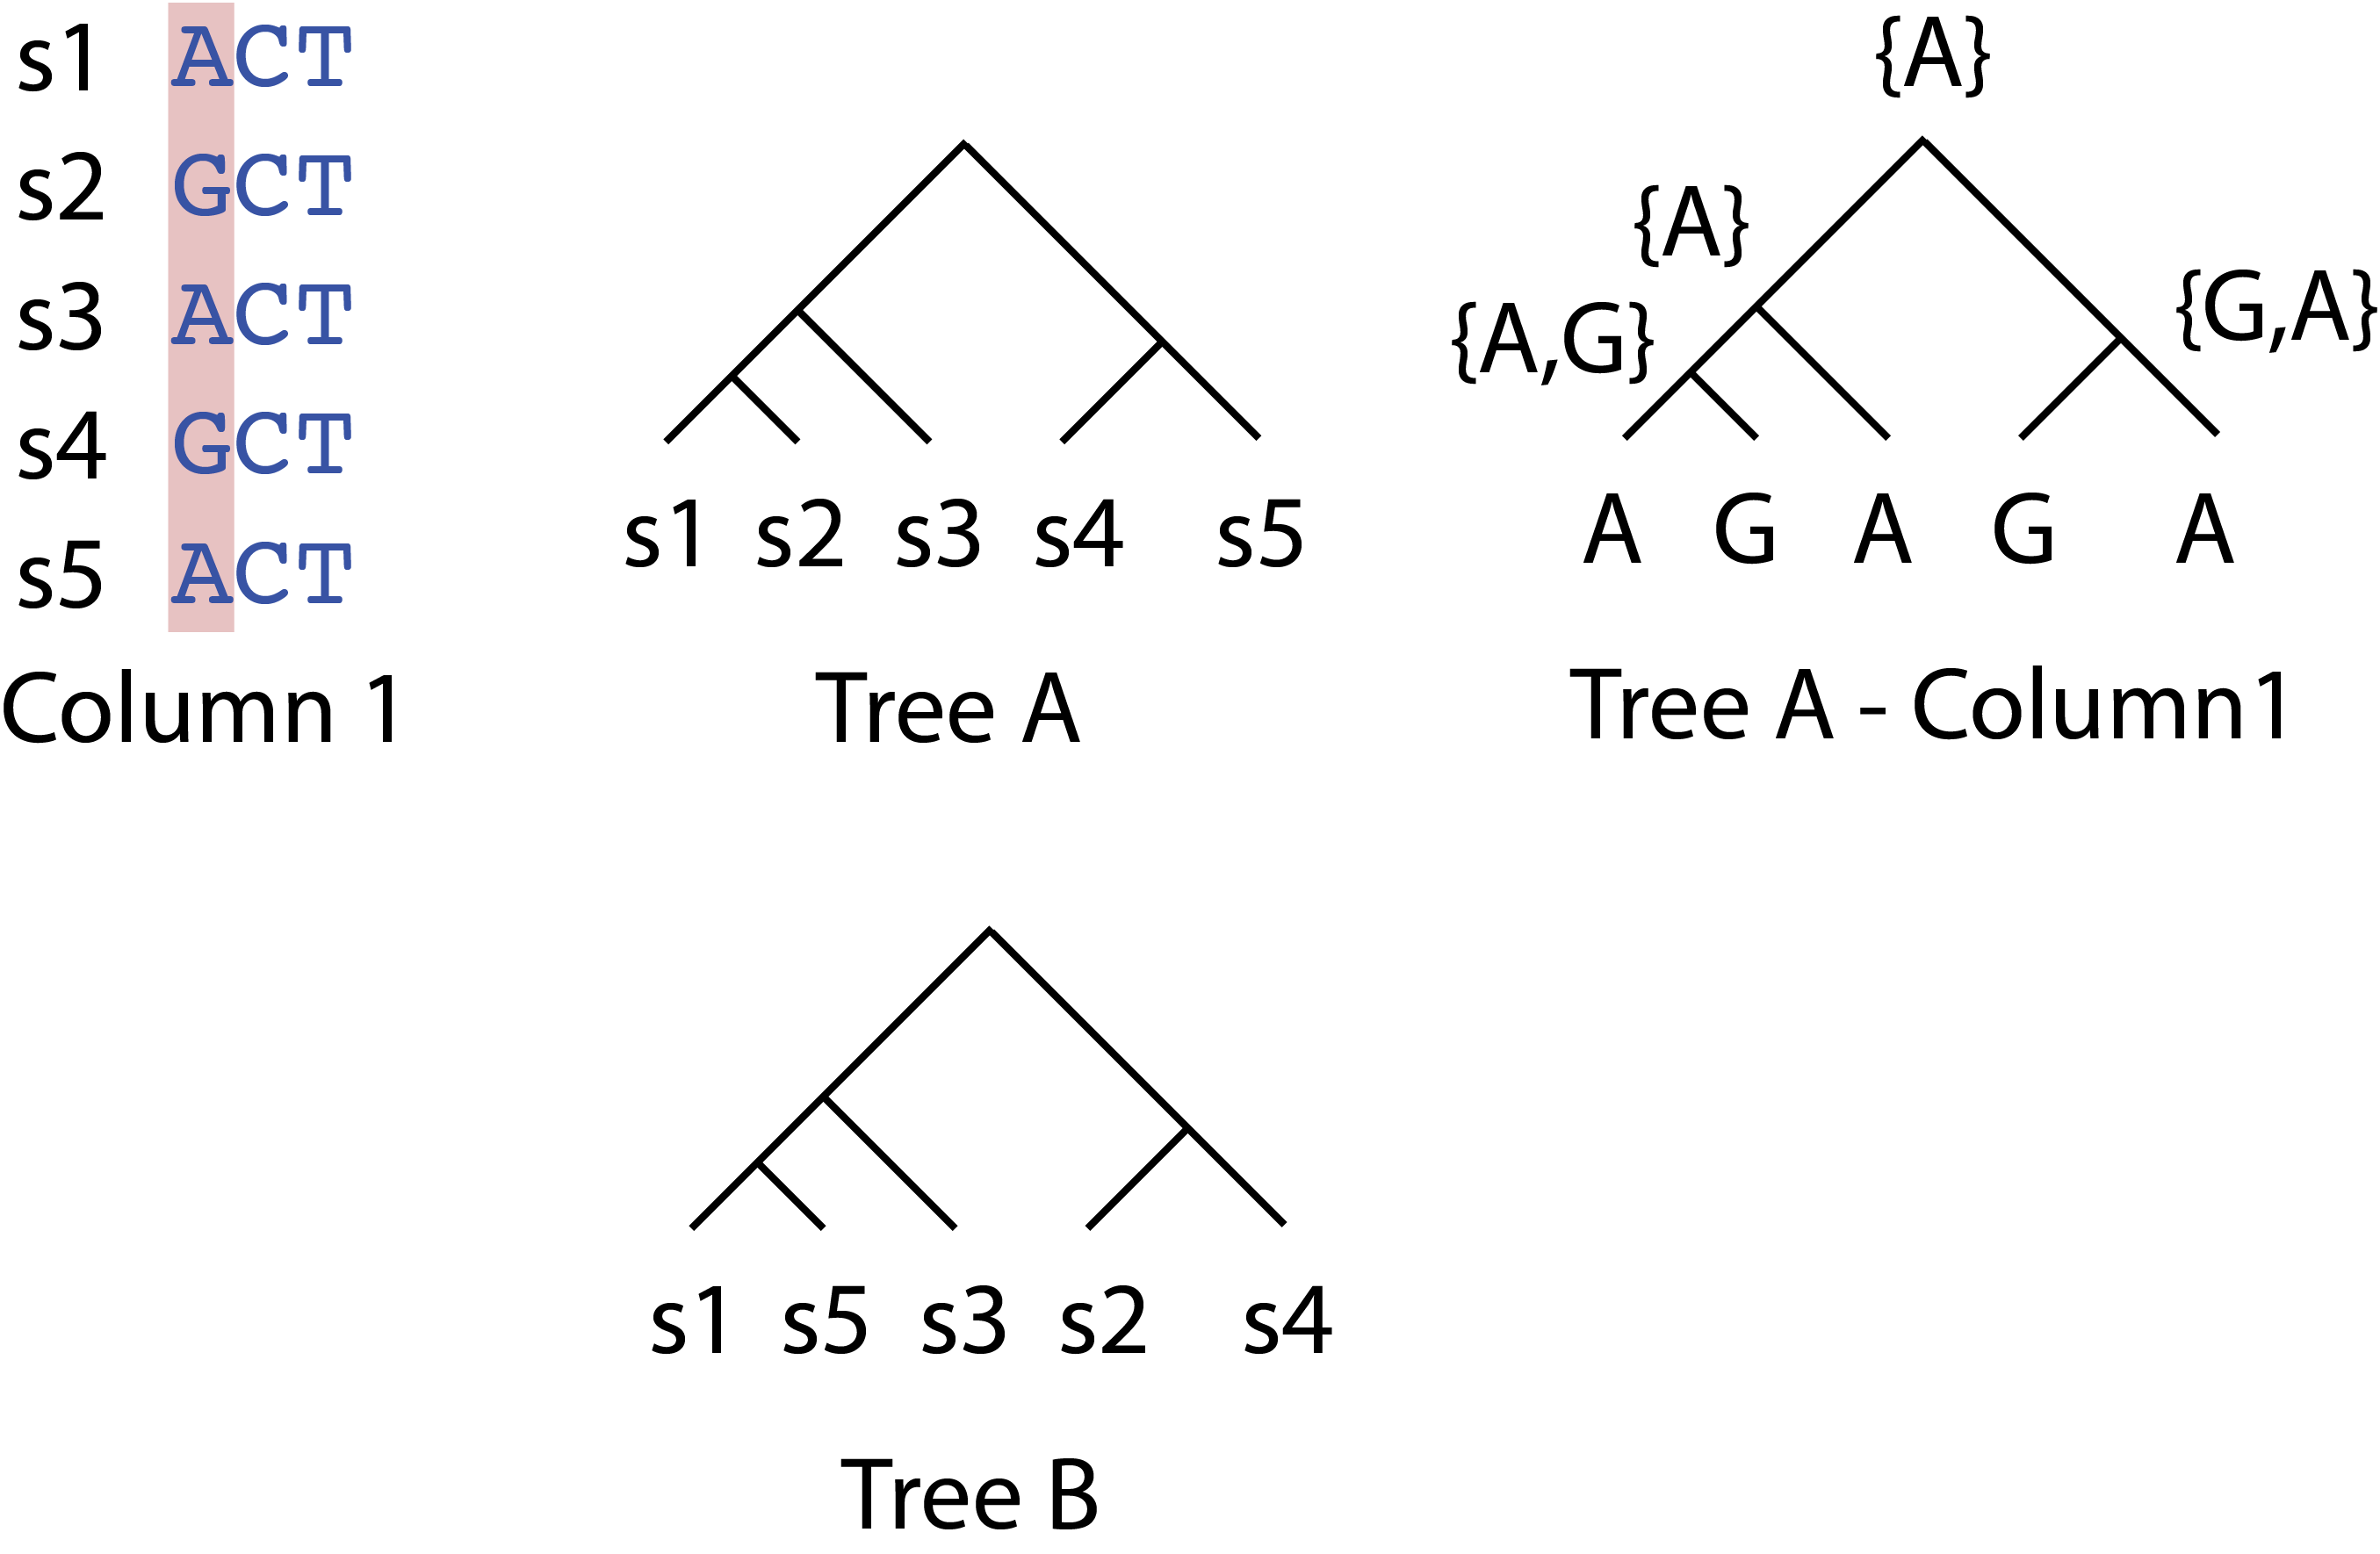
\includegraphics[width=0.5 \textwidth]{fig09/maximum_parsimony_tree_a.png}
\end{figure}

Use the first column of the MSA and also Tree A and B to answer the following questions.

\vspace{0.1 in}

\begin{parts}

%% (a)
  \part How many union operations are necessary to estimate the labels of the root and the internal nodes of Tree A?

\begin{solution}[0.35 in]
2
\end{solution}

%% (b)
  \part Estimate the labels of the root and the internal nodes of Tree B.
  
\begin{figure}[H]
      \centering
      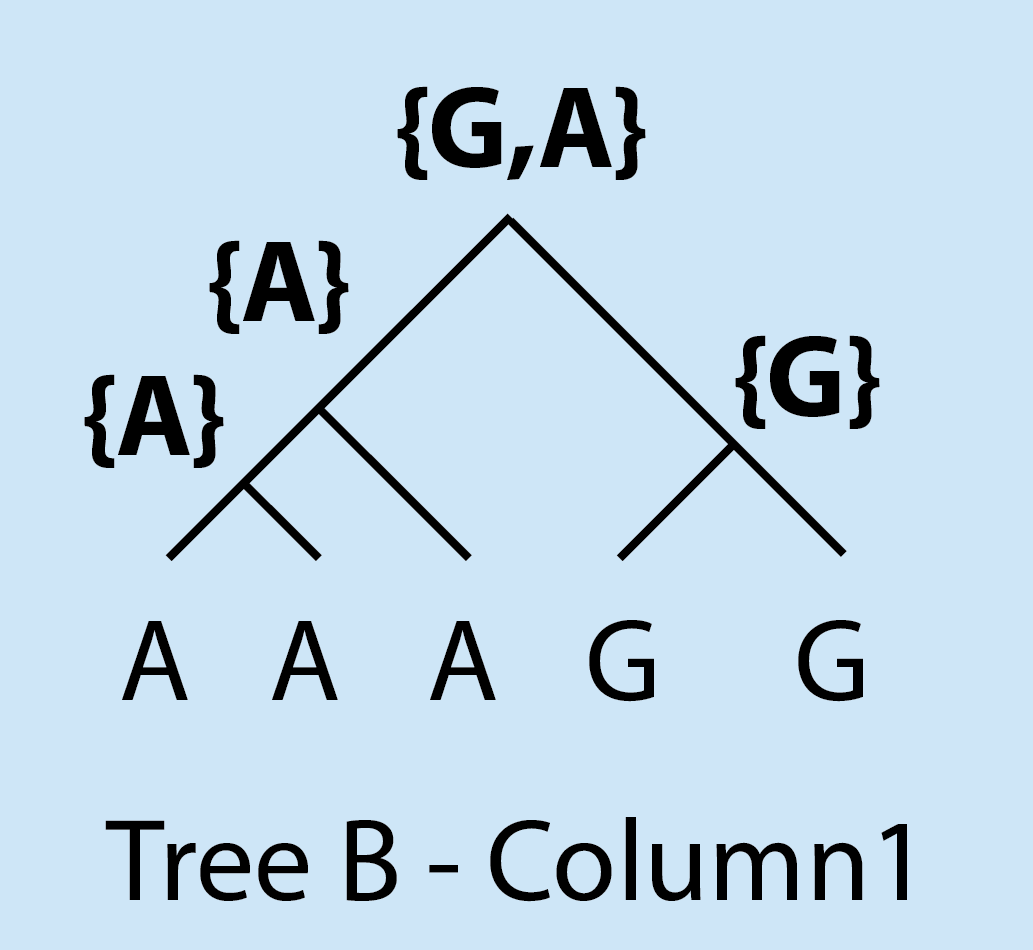
\includegraphics[width=0.2 \textwidth]{fig09/maximum_parsimony_tree_b_solution.png}
\end{figure}

%% (c)
  \part How many union operations are necessary to estimate the root and the internal nodes of Tree B?
  
\begin{solution}[0.35 in]
1
\end{solution}

%% (d)
  \part  Which tree, Tree A or B, indicates less evolutionary changes when only the first column is considered?
  
\begin{solution}[0.35 in]
Tree B
\end{solution}

  
\end{parts}



\end{questions}
%---------------------------------------------------------------------
       
\end{document}

